\section{Rotational Kinematics}

\begin{itemize}
    \item While objects can move in a straight line, objects can ALSO move in a circle
    \begin{itemize}
        \item Either an object is orbiting some point or something spins around some center
    \end{itemize}
    
    \item Instead of having position, velocity, and acceleration, we will have \textit{new} terms for moving in a circle instead
    \begin{itemize}
        \item \textbf{Angular position ($\theta$):} How much the object has rotated around the positive $x$-axis
        \item \textbf{Angular velocity ($\omega$):} How fast an object is going in a given direction at any point in the circle
        \begin{itemize}
            \item $\frac{d\theta}{dt} = \omega(t)$
            \item $\theta(t) = \int \omega \: dt$
        \end{itemize}
        \item \textbf{Angular acceleration ($\alpha$):} How fast an object changes it's velocity at any point in the circle of motion
        \begin{itemize}
            \item $\frac{d\omega}{dt} = \alpha(t)$
            \item $\omega(t) = \int \alpha \: dt$
        \end{itemize}
    \end{itemize}

    \item the kinematics equations from translational (standard) motion are the EXACT SAME equations in rotational kinematics, but we simply use the rotational kinematics variables instead of the translational kinematics variables
    
    \newpage
    \begin{definition}[Rotational Kinematics Equations]{def5.1.1:label}
        To calculate different values of 

        \[
        \begin{aligned}
            \omega_f &= \omega_i + \alpha t\\
            \Delta\theta &= \omega_it + \frac{1}{2}\alpha t^2\\
            \omega_f^2 &= \omega_i^2 + 2\alpha\Delta\theta
        \end{aligned}    
        \]
    \end{definition}

    \item it is important to note that values are \textbf{positive} if things move \textit{in the counterclockwise direction} and values are \textbf{negative} if things move \textit{in the clockwise direction}
    \item If you know the distance between the object moving in rotation and the center of rotation (in other words: the radius of the circle of rotation), then you can relate the rotational kinematics values with the translational kinematics values
    
    \begin{definition}[Rotational Kinematics $\leftrightarrow$ Translational Kinematics]{def5.1.2:label}
        \[
        S = \Delta\theta R    
        \]

        Where $S$ is the arc that the object travels around through a given angle $\theta$ and $R$ is the radius (the distance between the object and the center of rotation).

        \[
        v = \omega R    
        \]

        Where $R$ is the radius (the distance between the object and the center of rotation).

        \[
        a_{tangential} = \alpha R    
        \]

        Where $R$ is the radius (the distance between the object and the center of rotation). Note that this is the acceleration that is PENPENDICULAR to the acceleration that points towards the center of the circle.

        \[
        a_{centripetal} = \frac{v^2}{R} = \frac{\omega^2 R^2}{R} = \omega^2 R    
        \]

        Where $R$ is the radius (the distance between the object and the center of rotation). Note that this is the acceleration that points towards the CENTER of the circle. 
    \end{definition}
\end{itemize}


\begin{problem}
    A grinder rotates at 850RPM. Once the grinder turns off, it stops 3 minutes later. What is the angular acceleration and what is the final anglular position of the grinder?\\

    First, convert RPM to radians/second:

    \[
    850 \frac{\text{rev}}{\text{min}}\cdot\frac{2\pi \text{ radians}}{1 \text{ rev}}\cdot\frac{1 \text{ minute}}{60 \text{ seconds}} = 28.\bar{3} \frac{\text{radians}}{\s}   
    \]

    Now find angular acceleration:
    \[
    \alpha = \frac{\Delta \omega}{t} = \frac{\omega_f - \omega_i}{t} = \frac{- 28.3 \frac{\rad}{\s}}{60 \s} = -0.49 \frac{\rad}{\s^2}   
    \]

    Now find the final angular position:
    \[
    \begin{aligned}
        \omega_f^2 &= \omega_i^2 + 2\alpha\Delta\theta\\
        \theta_f &= \frac{\omega_f^2 - \omega_i^2}{2\alpha} + \theta_i\\
        \theta_f &= \frac{-(28.\bar{3} \frac{\rad}{\s})^2}{2(-0.49 \frac{\rad}{\s^2})}\\
        \theta_f &= 817.235 \rad
    \end{aligned}    
    \]
\end{problem}


\begin{problem}
    An object rotates and has a function that defines the angluar acceleration to be $\alpha(t) = 5t^3 - 4t$. You know that the initial rotational velocity is 5 $\frac{\rad}{\s}$ and the initial angular position is 2 radians. 

    \[
    \begin{aligned}
        \omega(t) &= \int_0^t \alpha(t)\:dt\\
        \omega(t) &= \int_0^t 5t^3 - 4t \: dt\\
        \omega(t) &= \frac{5}{4}t^4 - 2t^2 + 2
    \end{aligned}    
    \]
\end{problem}


\section{Moment of Inertia}

\textbf{Intertia} is the distribution of mass around the object's center of mass. This term allows us to differentiate between a disk and a chair that are both 5kg because up to this point we have tretaed those two objects as the same object. 


\section{Force, Energy, and Momentum in Rotation}

\begin{itemize}
    \item In the \textbf{linear world}, $KE = \frac{1}{2}mv^2$, but in the \textbf{rotational world} $KE = \frac{1}{2}I\omega^2$
    \item  In the \textbf{linear world}, $F = ma$, but in the \textbf{rotational world} $\tau = I\alpha$
    \begin{itemize}
        \item It shuold be noted that the above is Newton's Second Law just applied to rotation. Individual torques are $\tau_A = F_Ar\sin\theta$ where $r$ is the distance between the center of rotation and the point where the force is applied.
    \end{itemize}
    \item In the \textbf{linear world}, $W = F \cdot d$, but in the \textbf{rotational world} $W = \tau \cdot \theta$
    \item In the \textbf{linear world}, $P = Fv$, but in the \textbf{rotational world} $P = \tau\omega$
    \item In the \textbf{linear world}, $p = mv$, but in the \textbf{rotational world} $L = I\omega$
\end{itemize}

\begin{problem}
    \begin{center}
        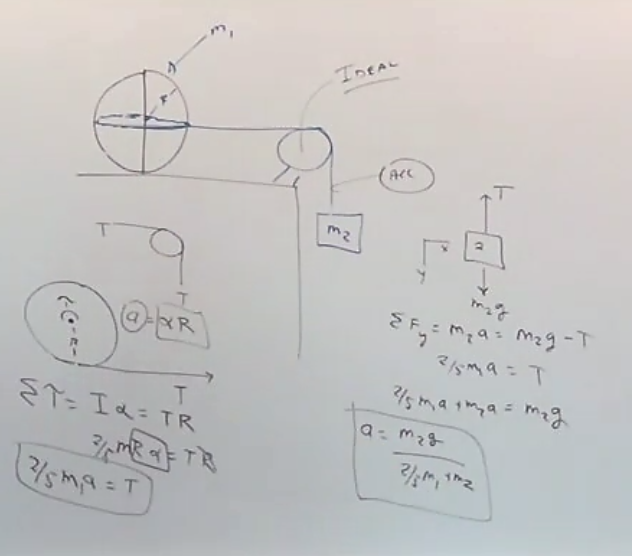
\includegraphics[width=0.75\textwidth]{chapters/ch5/images/fig5_1.PNG}
    \end{center}
\end{problem}

\begin{problem}
    \begin{center}
        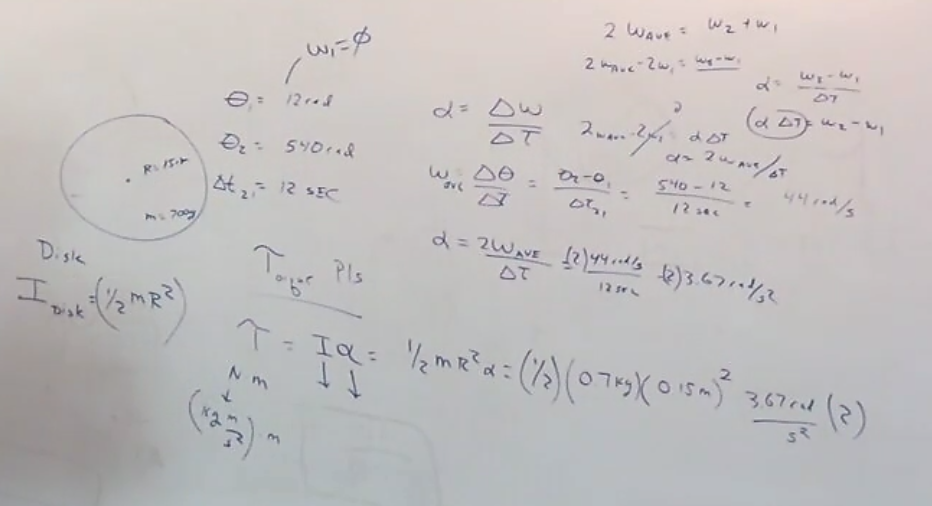
\includegraphics[width=0.75\textwidth]{chapters/ch5/images/fig5_2.PNG}
    \end{center}
\end{problem}


\section{Smooth Rolling Motion}

\[
\begin{aligned}
    \sum F_x  &= ma_{COM} = F_f\\
    \sum \tau_{NET} &= I\alpha = \tau_{APP} - \tau_f = \tau_{APP} - F_fR
\end{aligned}    
\]



\section{Newton's Second Law for Rotation}

\[
\begin{aligned}
    \tau &= I\alpha\\
    F_fR &= I\alpha\\
\end{aligned}    
\]


\section{Angular Momentum and Impulse}

\begin{itemize}
    \item We've been used to \textit{linear momentum} but there is also \textbf{angular momentum} that functions under the same properties
    
    \begin{definition}[Angular Momentum]{def5.6.1:label}
        \[
        L = I\omega     
        \]

        In every case in this class, \textbf{angular momentum will always be conserved}
    \end{definition}

    \item Angular momentum is the reason that an ice skater changes their speed
    \begin{itemize}
        \item When the skater holds out their arms, then the 
    \end{itemize}
\end{itemize}

\begin{problem}[Merry Go Round]
    \[
    \begin{aligned}
        L_i &= L_f\\
        I_m\omega_i &= I_m\omega_f + I_\parallel\omega_f\\
        \omega_f &= \frac{I_m\omega_i}{I_m + I_\parallel}
    \end{aligned}    
    \]
\end{problem}


\begin{problem}[Merry Go Round with Dog]
    \[
    \begin{aligned}
        L_i &= L_f\\
        I_m\omega_i + I_D\omega_i &= I_m\omega_f + I_D(\omega_f - \omega_D)
    \end{aligned}    
    \]
\end{problem}

\begin{itemize}
    \item Additionally, we can get an angular impulse similarly to how we get a linear impulse
    
    \begin{definition}[Angular Impulse]{def5.6.2:label}
        \[
        J_\angle = \tau_{AVG}\Delta T = I \Delta \omega      
        \]
    \end{definition}
\end{itemize}


\begin{problem}[Grindstone Problem]
    \[
    \begin{aligned}
        L_i &= L_f\\
        I_1\omega_i &= I_1\omega_f + I_2\omega_f\\
        I_1\omega_i &= \omega_f(I_1 + I_2)\\
        \omega_f &= \frac{I_1}{I_1+I_2}\omega_i\\
        \omega_f &= \frac{0.5M_1R_1^2}{0.5M_1R_1^2+0.5M_2R_2^2}\omega_i\\
    \end{aligned}    
    \]
\end{problem}